\chapter{Versiju vadība}

% Ievadiņš

Šajā darba nodaļā apskatīta versiju vadības sistēmu jeb VCS\nomenclature{VCS}{versiju vadības sistēma (angl. \textit{Version control system})} vēsture un pielietojums. VCS galvenais uzdevums ir saglabāt laika gaitā veiktās izmaiņas, kas veiktas ar datnēm. VCS ļauj arī atmest laika gaitā veiktās izmaiņas, atgriezties iepriekšējā stāvoklī, salīdzināt izmaiņas, redzēt kurš un kad ir veicis izmaiņas, kas atvieglo kļūdu atrašanu un to izlabošanu. Izmantojot VCS ir daudz grūtāk veikt neatgriezeniskas izmaiņas, piemēram, kļūdas pēc izdzēstu datni ir iespējams viegli atgūt.

\section{Versiju vadības sistēmu vēsture}
% No ProGit book
% Kad, kāpēc, kā strādā?
\subsection{Lokālas versiju vadības sistēmas}
Visvienkāršākā VCS, ko cilvēki mēdz izmantot ir vienkārša datņu pārkopēšana no vienas mapes citā, vai arī arhīvu veidošana. Šāds variants ir diezgan nedrošs, jo pieļauj cilvēcīgas kļūdas, piemēram, nepareizas datnes izmainīšanu. Tāpēc programmētāji radīja lokālu VCS, kas vienkāršā datubāzē saglabāja veiktās izmaiņas.
% Kaut kādi piemēri un gadi, attēls
\begin{figure}[H]%!ht
	\centering
	\captionsetup{justification=centering}
	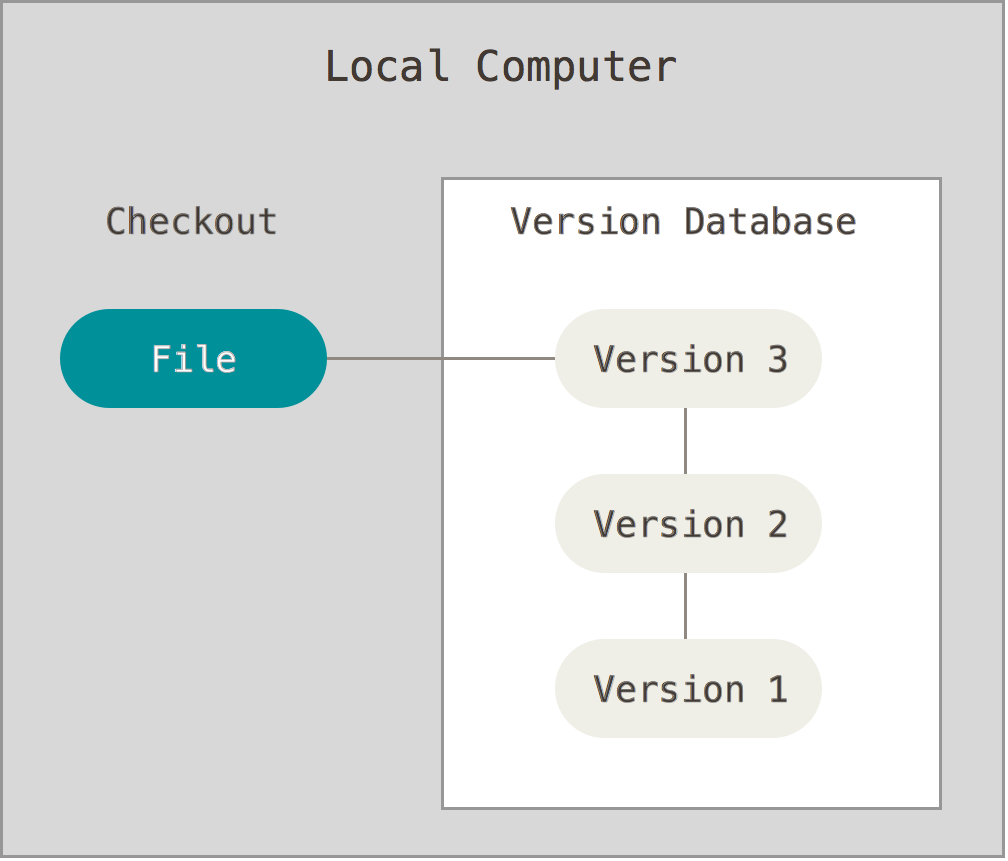
\includegraphics[width=1\textwidth]{local_version_control.png}
	\caption{Gitflow zarošanās stratēģijas attēlojums}
	\label{fig:gitflow-workflow}
\end{figure}

\subsection{Centralizētas VCS}
Lokālas VCS ir lieliskas, lai atvieglotu viena izstrādātāja darbu, bet ar lokālām VCS ir grūti vairākiem cilvēkiem sadarboties. Lai to atrisinātu tika radītas centralizētas VCS jeb CVCS\nomenclature{CVCS}{Centralizēta versiju vadības sistēma (angl. \textit{Centralized Version Control System})}. Šādām sistēmām, piemēram CVS, Subversion un Perforce, ir viens serveris uz kura atrodas visas datnes un no kura vairāki klienti tās paņem. Salīdzinot ar lokālām VCS, šādi būtiski uzlabojas spēja sadarboties. Tomēr CVCS sistēmām ir arī būtiskas problēmas. Visas datņu versijas atrodas tikai un vienīgi uz servera, bet klientam ir tikai tā versija, kuru tas paņēmis. Tāpēc, ja centrālais serveris atsakās darboties, izstrādātāju darbs praktiski tiek paralizēts, jo nav iespējams paņemt vai iesūtīt (angl. \textit{commit}) savas izmaiņas. Ja uz centrālā servera rodas datu bojājumi, ir iespējams pazaudēt visu projekta vēsturi, ja nav veikta VCS datubāzes dublēšana.
CVCS atvieglo sadarbību, bet tās centralizētais raksturs pieļauj projekta vēstures zaudēšanu, jo klientam ir tikai tā versija, ko tas paņēmis no centrālā servera.
\begin{figure}[H]%!ht
	\centering
	\captionsetup{justification=centering}
	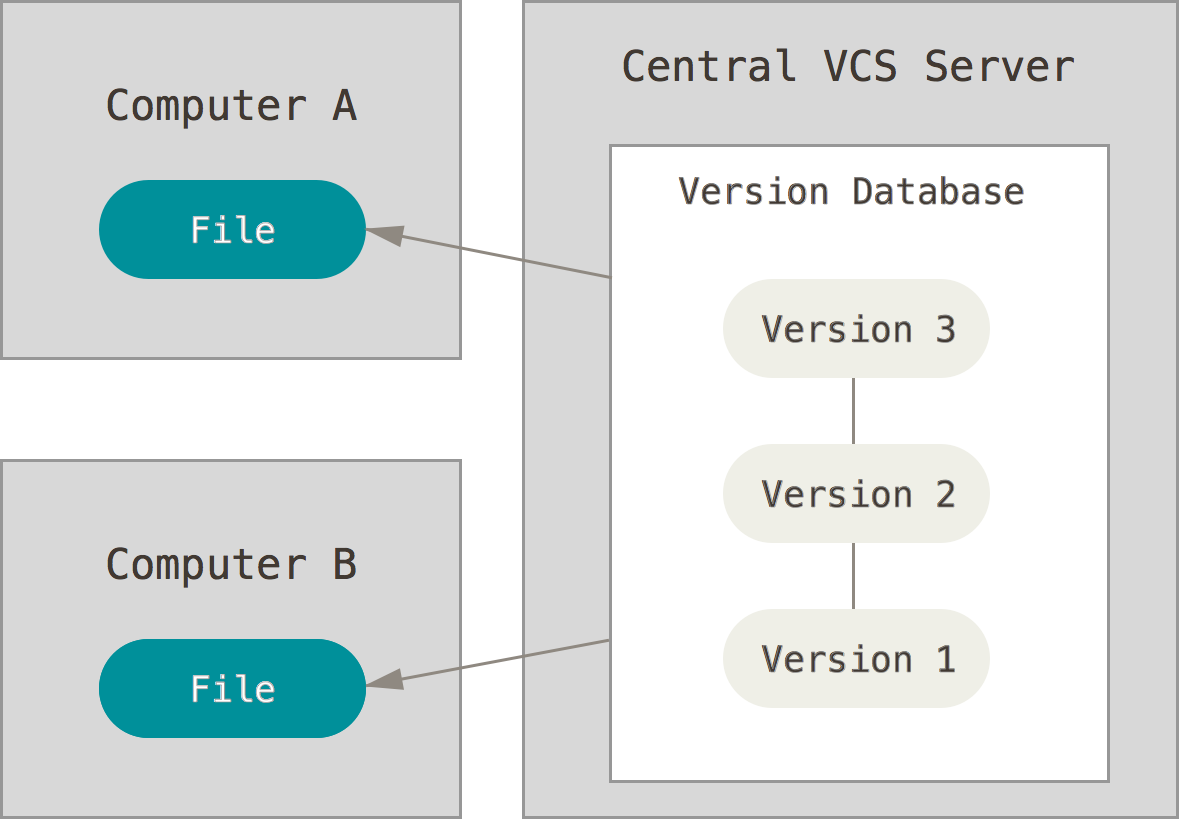
\includegraphics[width=1\textwidth]{centralized_version_control.png}
	\caption{Gitflow zarošanās stratēģijas attēlojums}
	\label{fig:gitflow-workflow}
\end{figure}

\subsection{Dalītas VCS}
CVCS problēmas atrisina dalītas VCS jeb DVCS\nomenclature{DVCS}{dalīta versiju vadības sistēma (angl. \textit{Distributed Version Control System})}. DCVS sistēmās, kā Git, Mercurial, Bazaar, Darcs joprojām izmanto centralizētu serveri, uz kura klienti iesūta savas izmaiņas, bet atšķirībā no CVCS, klienti nepaņem tikai datņu pēdējās versijas, bet pilnībā visu projekta vēsturi. Tādejādi, galvenajam serverim atsaktoties darboties, projekta vēsturi ir iespējams atjaunot no jebkura klienta.
\begin{figure}[H]%!ht
	\centering
	\captionsetup{justification=centering}
	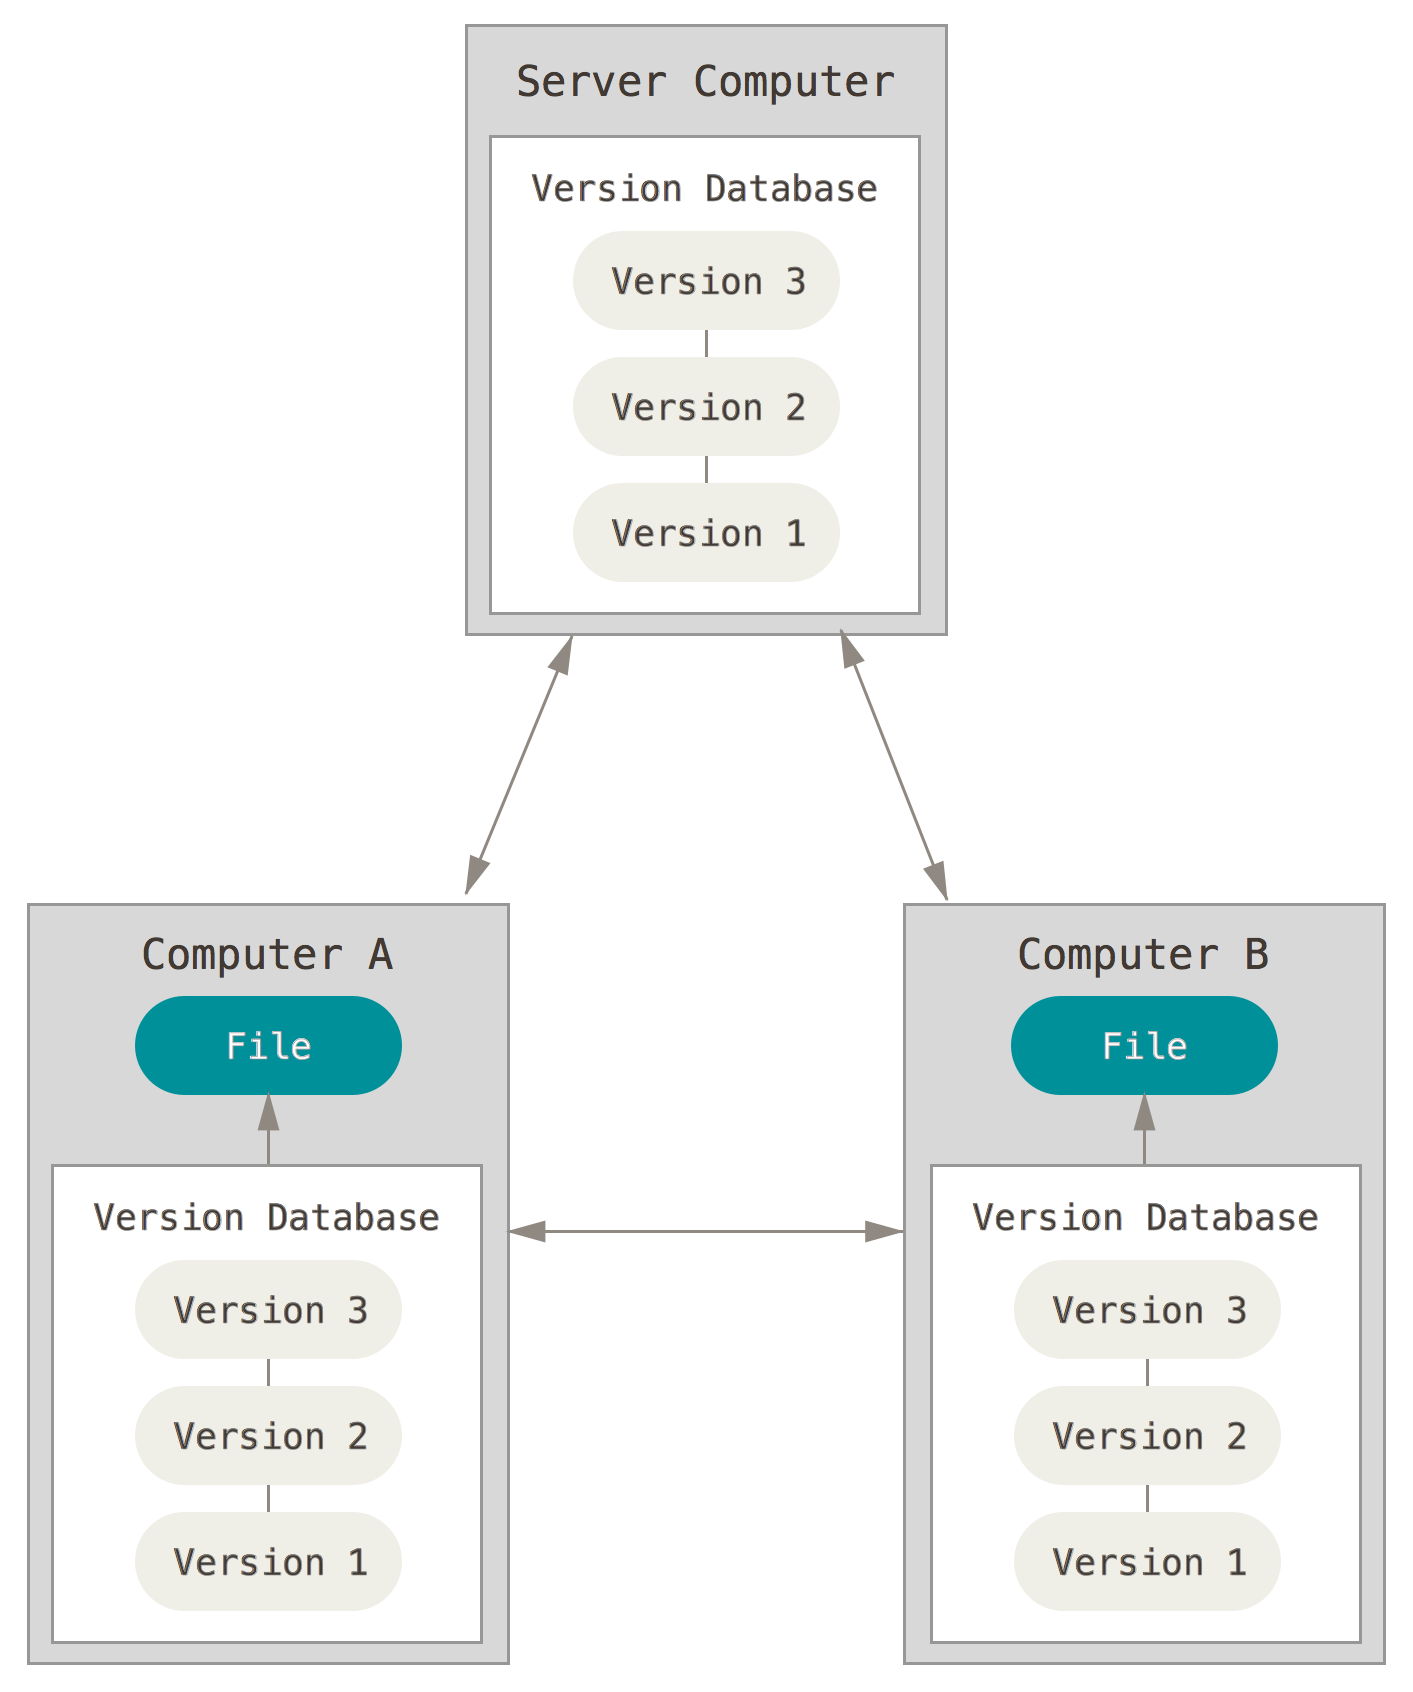
\includegraphics[width=1\textwidth]{distributed_version_control.png}
	\caption{Gitflow zarošanās stratēģijas attēlojums}
	\label{fig:gitflow-workflow}
\end{figure}

\section{Versiju vadības sistēma Git}
% Kas ir repo?
Darbā izmantota Git versiju kontrole. ... % Vēl ko vajag
Git ir DVCS, ko 2005. gadā radīja Linus Torvals kopā ar Linux kodola (angl. \textit{Linux kernel}) izstrādātāju komandu, lai aizvietotu trešās puses DVCS BitKeeper, kuras autori BitMover 2005. gadā izlēma vairs nepiedāvāt bezmaksas versijas Linux kodola izstrādātājiem. Tāpēc Linux kodola izstrādātāji nolēma radīt savu VCS, ko izmantot Linux kodola versiju vadībai. Galvenie mērķi jaunajai sistēmai bija, lai tā būtu ātra, pilnībā dalīta, spētu efektīvi apstrādāt lielus projektus un atbalstītu nelineāru izstrādi.

\subsection{Kā strādā Git}
Git piedāvā līdzīgu lietotāja saskarni kā citas VCS, bet iekšienē Git datus uztver savādāk nekā citas VCS. Lielākā daļa VCS saglabā veikto izmaiņu sarakstu, attiecīgi kā datnes un to izmaiņas, jeb deltas.
% Attēls https://git-scm.com/book/en/v2/Getting-Started-Git-Basics
Toties Git katru versiju uztver gluži kā failu sistēmas momentuzņēmumu. Katra saglabātā versija saglabā esošo projekta stāvokli un, lai sistēma būtu efektīvāka, uz datnēm kuras nav mainītas Git izveido atsauces. Git, uztverot versijas kā failu sistēmas momentuzņēmumus, atļauj ļoti efektīvi veidot nelineāras darbplūsmas (angl. \textit{Workflow}).
% Attēls un arī varētu piemēru no Pluralsight video.
Vēl viens būtisks ieguvums no DVCS ir tas, ka lielākā daļa darbību ir iespējams izdarīt lokāli, bezsaistē. Tas nozīmē, ka Git ir ļoti ātrs, jo nav nekāds tīkla virstēriņš lielākajai daļai darbību, kas ir tipisks CVCS.
% Nearly every operation is local

Integritāte
Pirms Git saglabā datus, tas visam izveido SHA-1 kontrolsummu (angl. \textit{Checksum}) un pēc tam veido atsauces izmantojot izveidotās kontrolsummas. Savā datubāzē Git saglabā visu pēc datņu satura kontrolsummas, nevis pēc to nosaukuma. Tas nozīmē, ka ir neiespējami izdarīt izmaiņas tā, lai Git par tām nezinātu. Tā Git spēj atklāt datu bojājumus, kas radušies tīkla vai cietā diska bojājumu gadījumā. Kā arī, praktiski visas Git darbības tikai pievieno datus datubāzē, tāpēc bieži ir iespējams atgūt datus, kuri šķiet neatgriezeniski pazaudēti.

Trīs stāvokļi
Staging - Ļauj sagatavot savu ``Commit''. Iespējams iekļaut tikai daļu no savām izmaiņām.

\subsection{Zarošanās}
Zarošanās (angl. \textit{Branching})
Git zarošanās ir ļoti spējīgs mehānisms, kas ļauj veikt eksperimentus it nemaz netraucējot jau uzrakstītajam kodam.
\subsubsection{Izvēlētā zarošanās stratēģija}
% http://nvie.com/posts/a-successful-git-branching-model/
% https://www.atlassian.com/git/tutorials/comparing-workflows/gitflow-workflow
Darbā izvēlēts izmantot Gitflow darbplūsmu, kas ir īpaši lietderīga lieliem projektiem, jo Gitflow darbplūsma skaidri nosaka repozitorija zaru funkcijas. Gitflow pamatā galvenie ir divi zari: pamatzars (angl. \textit{master}) un izstrādes zars(angl. \textit{develop}). Pamatzars atspoguļo relīžu vēsturi un koda iesūtījumi ir atzīmēti ar versiju numuriem. Ikreizi, kad pamatzarā tiek veikta kāda izmaiņa, to jāatzīmē ar jaunu versijas numuru. Izstrādes zars kalpo pievienotās funkcionalitātes integrācijai. Tomēr, katrai pievienotajai iespējai vajadzētu atrasties savā funkcionalitātes (angl. \textit{feature}) zarā. Citās darbplūsmās parasti atzarojas no pamatzara, bet Gitflow darbplūsmā atzarošanās tiek veikta no izstrādes zara. Katra jaunā iespēja atzarojas no izstrādes zara un kad tā ir pabeigta, tā tiek sapludināta (angl. \textit{merge}) ar izstrādes zaru.
Kad pienāk laiks jaunai relīzei, no izstrādes zara atzarojas relīzes zars. Relīžu zaros nekad netiek pievienota jauna funkcionalitāte. Relīzes zari tiek tikai izmantoti tālākai koda sagatavošanai nākamajai versijai, tajā veic tikai labojumus. Tajā nepievieno papildus funkcionalitāti. Kad relīze ir gatava, to sapludina ar pamatzaru, atzīmē ar jaunu versijas numuru un sapludina arī ar izstrādes zaru.
Apkopes (angl. \textit{maintenance}) zari tiek izmantoti, lai ātri veiktu labojumus relīzēm. Apkopes zars atzarojas no pamatzara un tiklīdz labojums ir pabeigts, tas tiek sapludināts ar pamatzaru un izstrādes zaru, vai vēl neizlaistu relīzes zaru.
Šāda vairākzaru darbplūsma ļauj izstrādei neapstāties pie viena uzdevuma, piemēram, nespiež strādāt tikai pie relīzes vai papildu funkcionalitātes izstrādes. Tā kā ir vairāki zari gan relīzēm, gan funkctionalitātei, komandas var strādāt paralēli, katra pie sava uzdevuma nebojājot repozitoriju citām komandām.
\begin{figure}[H]%!ht
	\centering
	\captionsetup{justification=centering}
	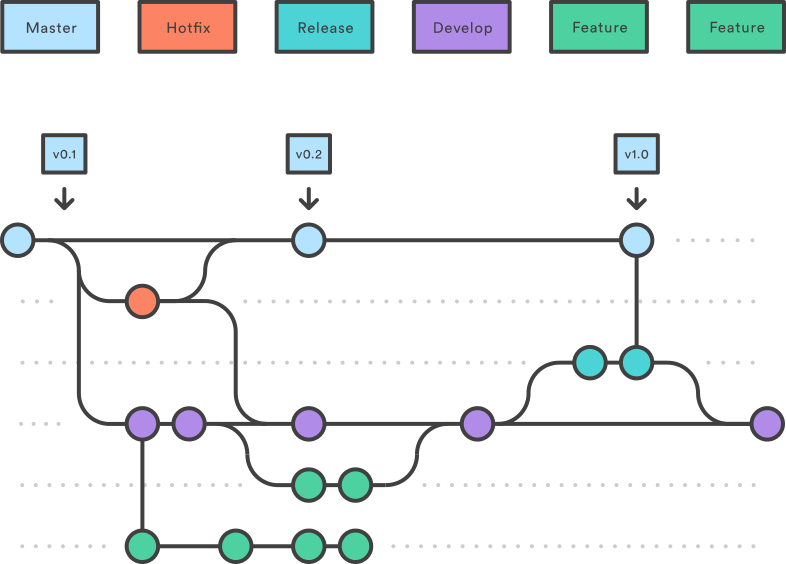
\includegraphics[width=1\textwidth]{gitflow_workflow.png}
	\caption{Gitflow zarošanās stratēģijas attēlojums}
	\label{fig:gitflow-workflow}
\end{figure}
Master zars atspoguļo to mājaslapas kodu, kas strādās uz RaspberryPi servera. Tiklīdz kā tikt atjaunināts master zars, serveris to lejuplādēs un sāks izmantot jaunāko koda relīzi.
Develop zars izmantots izmaiņu integrēšanai.
Galvenais darbs notiks uz feature zariem, kuros fokusēti tiks nodalīta laika gaitā pievienotā funkcionalitāte.



Darba praktiskā daļa ir sadalīta divos repozitorijos. Viens repozitorijs - piekļuves sistēmas administrēšanas mājaslapai, otrs - infrastruktūras uzstādīšanai izmantojot Chef.

\section{Infrastruktūra kā kods}
